\documentclass{sigchi}

% Use this section to set the ACM copyright statement (e.g. for
% preprints).  Consult the conference website for the camera-ready
% copyright statement.

% Copyright
\CopyrightYear{2020}
%\setcopyright{acmcopyright}
\setcopyright{acmlicensed}
%\setcopyright{rightsretained}
%\setcopyright{usgov}
%\setcopyright{usgovmixed}
%\setcopyright{cagov}
%\setcopyright{cagovmixed}
% DOI
\doi{https://doi.org/10.1145/3313831.XXXXXXX}
% ISBN
\isbn{978-1-4503-6708-0/20/04}
%Conference
\conferenceinfo{CHI’20,}{April  25--30, 2020, Honolulu, HI, USA}
%Price
\acmPrice{\$15.00}

% Use this command to override the default ACM copyright statement
% (e.g. for preprints).  Consult the conference website for the
% camera-ready copyright statement.

%% HOW TO OVERRIDE THE DEFAULT COPYRIGHT STRIP --
%% Please note you need to make sure the copy for your specific
%% license is used here!
% \toappear{
% Permission to make digital or hard copies of all or part of this work
% for personal or classroom use is granted without fee provided that
% copies are not made or distributed for profit or commercial advantage
% and that copies bear this notice and the full citation on the first
% page. Copyrights for components of this work owned by others than ACM
% must be honored. Abstracting with credit is permitted. To copy
% otherwise, or republish, to post on servers or to redistribute to
% lists, requires prior specific permission and/or a fee. Request
% permissions from \href{mailto:Permissions@acm.org}{Permissions@acm.org}. \\
% \emph{CHI ‘16},  May 07--12, 2016, San Jose, CA, USA \\
% ACM xxx-x-xxxx-xxxx-x/xx/xx\ldots \$15.00 \\
% DOI: \url{http://dx.doi.org/xx.xxxx/xxxxxxx.xxxxxxx}
% }

% Arabic page numbers for submission.  Remove this line to eliminate
% page numbers for the camera ready copy
% \pagenumbering{arabic}

% Load basic packages
\usepackage{balance}       % to better equalize the last page
\usepackage{graphics}      % for EPS, load graphicx instead 
\usepackage[T1]{fontenc}   % for umlauts and other diaeresis
\usepackage{txfonts}
\usepackage{mathptmx}
\usepackage[pdflang={en-US},pdftex]{hyperref}
\usepackage{color}
\usepackage{booktabs}
\usepackage{textcomp}

% Some optional stuff you might like/need.
\usepackage{microtype}        % Improved Tracking and Kerning
% \usepackage[all]{hypcap}    % Fixes bug in hyperref caption linking
\usepackage{ccicons}          % Cite your images correctly!
\usepackage[utf8]{inputenc} % for a UTF8 editor only
\usepackage{listings}

% If you want to use todo notes, marginpars etc. during creation of
% your draft document, you have to enable the “chi_draft” option for
% the document class. To do this, change the very first line to:
% “\documentclass[chi_draft]{sigchi}”. You can then place todo notes
% by using the “\todo{...}”  command. Make sure to disable the draft
% option again before submitting your final document.
\usepackage{todonotes}

% Paper metadata (use plain text, for PDF inclusion and later
% re-using, if desired).  Use \emtpyauthor when submitting for review
% so you remain anonymous.
\def\plaintitle{Space Folding in Virtual Reality}
\def\plainauthor{Joe Strout}
\def\emptyauthor{}
\def\plainkeywords{virtual reality;travel;nonphysical spaces}
\def\plaingeneralterms{Virtual Reality}

% llt: Define a global style for URLs, rather that the default one
\makeatletter
\def\url@leostyle{%
  \@ifundefined{selectfont}{
    \def\UrlFont{\sf}
  }{
    \def\UrlFont{\small\bf\ttfamily}
  }}
\makeatother
\urlstyle{leo}

% To make various LaTeX processors do the right thing with page size.
\def\pprw{8.5in}
\def\pprh{11in}
\special{papersize=\pprw,\pprh}
\setlength{\paperwidth}{\pprw}
\setlength{\paperheight}{\pprh}
\setlength{\pdfpagewidth}{\pprw}
\setlength{\pdfpageheight}{\pprh}

% Make sure hyperref comes last of your loaded packages, to give it a
% fighting chance of not being over-written, since its job is to
% redefine many LaTeX commands.
\definecolor{linkColor}{RGB}{6,125,233}
\hypersetup{%
  pdftitle={\plaintitle},
% Use \plainauthor for final version.
%  pdfauthor={\plainauthor},
  pdfauthor={\emptyauthor},
  pdfkeywords={\plainkeywords},
  pdfdisplaydoctitle=true, % For Accessibility
  bookmarksnumbered,
  pdfstartview={FitH},
  colorlinks,
  citecolor=black,
  filecolor=black,
  linkcolor=black,
  urlcolor=linkColor,
  breaklinks=true,
  hypertexnames=false
}

% create a shortcut to typeset table headings
% \newcommand\tabhead[1]{\small\textbf{#1}}

% End of preamble. Here it comes the document.
\begin{document}

\title{\plaintitle}

\numberofauthors{1}
\author{%
  \alignauthor{Joe Strout\\
    \affaddr{Colorado State University}\\
    \affaddr{Fort Collins, United States}\\
    \email{joe@strout.net}}\\
}

\maketitle

\begin{abstract}
  UPDATED---\today. Real walking is a desireable way to navigate a virtual environment (VE), but is limited by the amount of physical space in which the user can walk.  Many attempts to overcome this limitation provide only modest gains in VE size, or don’t reduce the physical space enough to work in a typical home environment, or don’t allow the user to freely explore.  This study presents a new approach, \textit{space folding}, which connects multiple virtual spaces via portals in such a way that they occupy the same physical space.  This allows the user to use natural walking to navigate an arbitrarily large VE in a physical space as small as $2 m \times 3 m$.  To begin evaluating the effectiveness of the technique, a pilot study was conducted.  Five subjects each performed a task collecting stars in a 5-room ($60 m^2$) VE folded into a $3 m \times 4 m$ ($12 m^2$) physical space, then completed an exit survey and the NASA TLX.  Results suggest that users are able to easily navigate the folded space, and enjoyed the ability to freely navigate it via real walking.
\end{abstract}


% ACM Classfication

\begin{CCSXML}
<ccs2012>
<concept>
<concept_id>10003120.10003121.10003124.10010866</concept_id>
<concept_desc>Human-centered computing~Virtual reality</concept_desc>
<concept_significance>500</concept_significance>
</concept>
</ccs2012>
\end{CCSXML}

\ccsdesc[500]{Human-centered computing~Virtual reality}


\begin{CCSXML}
<ccs2012>
<concept>
<concept_id>10003120.10003121.10003124.10010866</concept_id>
<concept_desc>Human-centered computing~Virtual reality</concept_desc>
<concept_significance>500</concept_significance>
</concept>
<concept>
<concept_id>10003120.10003121</concept_id>
<concept_desc>Human-centered computing~Human computer interaction (HCI)</concept_desc>
<concept_significance>100</concept_significance>
</concept>
<concept>
<concept_id>10010147.10010371.10010387.10010866</concept_id>
<concept_desc>Computing methodologies~Virtual reality</concept_desc>
<concept_significance>300</concept_significance>
</concept>
</ccs2012>
\end{CCSXML}

\ccsdesc[500]{Human-centered computing~Virtual reality}
\ccsdesc[100]{Human-centered computing~Human computer interaction (HCI)}
\ccsdesc[300]{Computing methodologies~Virtual reality}

% Author Keywords
\keywords{\plainkeywords}

% Print the classficiation codes
\printccsdesc



\section{Introduction}

Real walking is widely regarded as the most natural and direct travel technique.  It provides vestibular cues, requires no training, promotes spatial understanding, and is especially efficient at maneuvering tasks.  However, it is not widely adopted in consumer VR applications primarily because of the limits of the user’s physical area.  Current consumer headsets are designed for indoor use only, and most users do not have an indoor space larger than a few meters on a side.

While many approaches have been developed to “compress” a larger virtual space into a smaller physical one (see Related Work), various limitations make these difficult to apply to a room-scale VR setup of say 3 by 4 meters area, or limit the amount of extra space gained to a modest factor of less than 2X.

This study introduces an approach to spatial compression that allows for any compression factor, works in a space as small as 2 by 3 meters, and works with completely natural walking, without redirection.  Of course there are always trade-offs; the technique presented works best for indoor virtual scenes, and makes no attempt to keep the user from noticing the spatial manipulation.  An experiment is presented to show that this does not detract from the user’s ability to navigated the virtual environment, or in overall user satisfaction.


\begin{figure*}[htb]
  \centering
  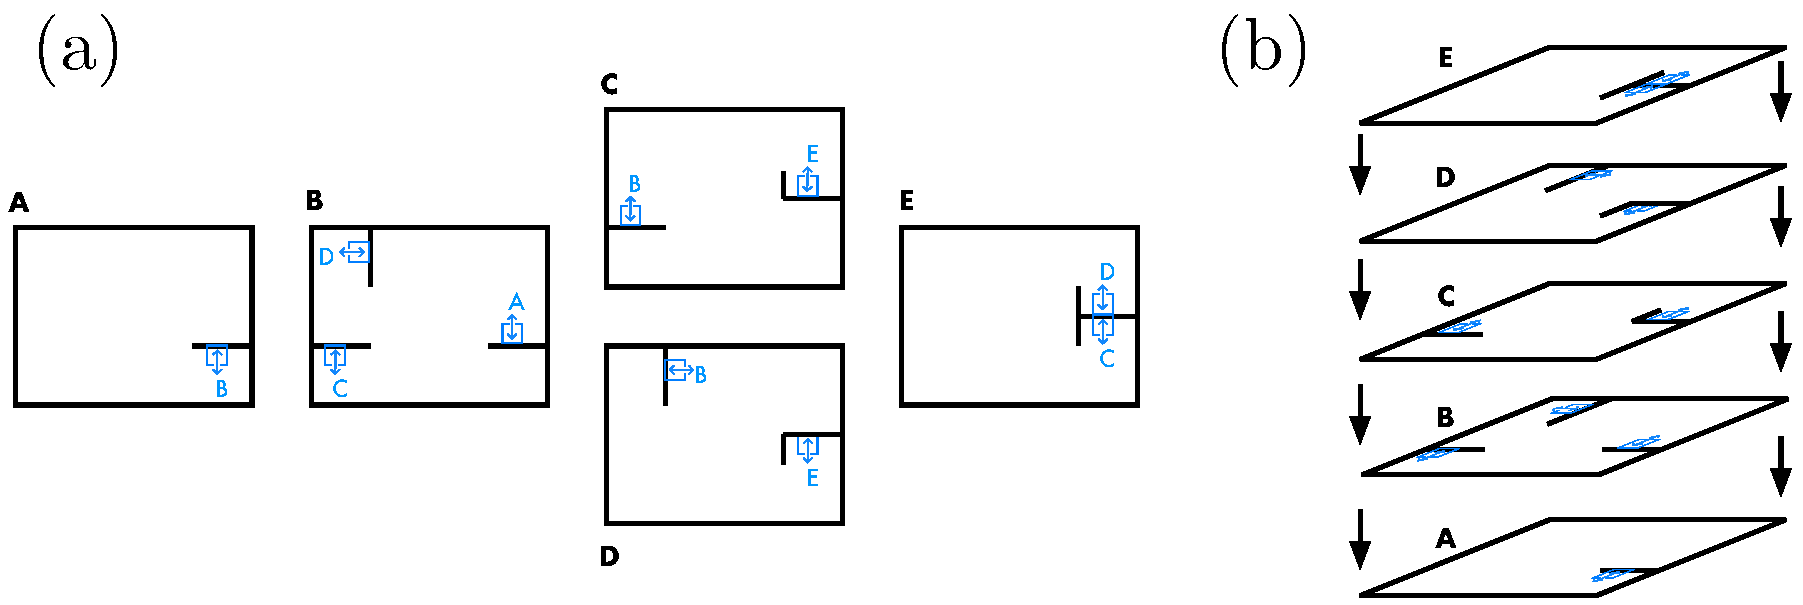
\includegraphics[width=1.75\columnwidth]{figures/FoldingDiagram.pdf}
  \caption{Illustration of the space folding technique.  Each “room” of the virtual environment contains portals that connect to other rooms, allowing both viewing and travel in both directions.  The layout shown here was used in the pilot study.  In (a) the five rooms are shown in top-down view, separated for clarity; (b) illustrates how these virtual spaces are “folded” into one physical space.}~\label{fig:foldingDiagram}
\end{figure*}

\section{Related Work}

Vaslevska \& Kaufman~\cite{vasylevska2017compressing} reviewed several techniques for compressing virtual environments to enable natural locomotion within a limited physical space.  In all those techniques, but unlike the present approach, keeping the user from noticing the manipulation was a primary goal.

Field and Vamplew~\cite{field2004generalised} extended earlier redirected walking work with additional algorithms to redirect the user to the center of the physical space, and to keep the user on circular paths that anticipate possible future turns.  A more recent review by Nilsson et al~\cite{nilsson201815} covered 15 years of redirected walking research, summarizing the state of the field in 2018.  All variations on this approach require substantial space, as confirmed by Hodgson and Bachmann~\cite{hodgson2013comparing}.  Subjects walked within a 25m x 45m facility under either normal conditions, or while using redirection.  The authors also did simulations of agents moving at 1m/s, considered typical of VR users.  Their experiments determined that a 35m x 35m space would be needed for such locomotion in an unconstrained virtual environment.

A very different approach to compressing a virtual environment is change blindness redirection, explored by Suma et al~\cite{suma2011leveraging}.  With this technique, the layout of some part of the VE is changed when the user isn’t looking at it.  For example, a doorway may be moved from one wall to another while the user is looking away or their view is occluded.  The technique produces a powerful illusion of a large VE, but requires the user to follow particular paths; it does not allow for free exploration.

Suma and Krum introduced the term \textit{impossible spaces} to describe a closely related technique, in which rooms are spatially expanded while not in view, thus producing a self-overlapping architecture~\cite{suma2012impossible}.  The authors were intent on maintaining the illusion of a natural space, and found that rooms could overlap by as much as 56\% before users began to notice.  The present work could be considered an extreme version of impossible spaces, in which the objective to keep users from noticing is abandoned, and a much higher overlap factor is obtained.

While many spatial compression studies focus on measuring the ability of users to detect the manipulation, Peck et al~\cite{peck2011evaluation} instead compared several measures of navigability for redirected walking (with distractors to create redirection opportunities), walking-in-place, and joystick locomotion.  While the present study does not include direct comparisons of travel methods, this would be a promising direction for future research.


\section{Methods}

\subsection{Technique}

An illustration of the VR Space Folding technique is shown in Figure~\ref{fig:foldingDiagram}.  The central idea is relatively simple: the virtual environment (VE) is divided into spaces (“rooms”), joined by portals.  Stepping through a portal takes the user to a different virtual space, which occupies the same physical space as the previous room.  In this way, an arbitrarily large VE can be “folded” into a restricted physical environment.

While the core idea would work with opaque portals, the experience is enhanced by portals that can be seen through.  For example, when standing in the southeast corner of the physical space while in room $A$ of Figure~\ref{fig:foldingDiagram} (assuming north is towards the top of the diagram), and looking north, one would see part of room $B$, just as if looking through an ordinary arch or open doorway.  Stepping through that doorway, and then turning around and looking south, one would see the corner of room $A$ just vacated.

The technique places two important constraints on the placement of the connecting portals:

\begin{enumerate}
\item Because the user must be able to physically walk through them, portals may not be placed on the outside boundary of the physical space.  Instead they must turned perpendicular to that boundary, or otherwise moved away from the outside edge so that the user has room to walk on both sides of each portal.

\item Each portal has a specific location in physical space, which must be the same as its position in \textit{both} virtual spaces it connects.  We cannot, for example, connect the west side of one room to the east side of another.
\end{enumerate}

However, within these constraints, portal placement is otherwise free.  In this pilot study we have placed all portals orthogonal to the room walls, but that is not necessary.  Within a single virtual room, a portal is one-sided, as in the aforementioned portal between rooms A and B; this is traversed only northward from room A, or southward from room B.  But two portals may be placed back-to-back, as illustrated by the portals from room E to rooms C and D.  In this example, looking through the archway from the south one would see room C; but looking through it from the north, one would see room D.

Graph theory is helpful to understand the design space of the folded VE.  The set of connected virtual rooms form an undirected, connected graph.  The graph size is the number of rooms, and its order is equal to the largest number of portals in any room.  In most applications this order is likely to be relatively low, as each portal takes up roughly $2 m^2$ of physical space.  We can therefore enumerate the possible room graphs.  An order 1 graph (i.e. no more than one portal per room) is always exactly two rooms.  There are two possible order 2 (two portals per room) graphs, regardless of size: either all rooms connected in a line, or the end rooms also joined to form a loop.

\begin{figure}[htb]
  \centering
  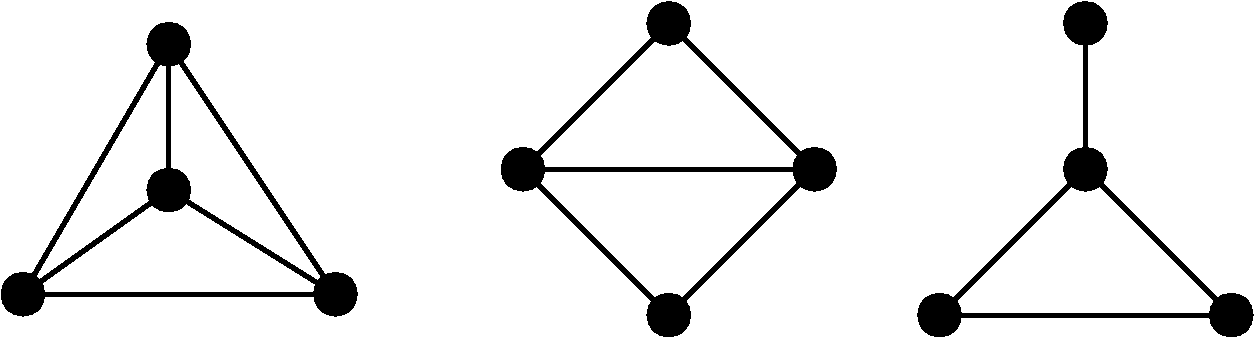
\includegraphics[width=1\columnwidth]{figures/Size4Graphs.pdf}
  \caption{All possible order-3 graphs of 4 nodes.  These are the possible topologies for a VE with 4 rooms and up to 3 doors per room.}~\label{fig:size4Graphs}
\end{figure}

\begin{figure}[htb]
  \centering
  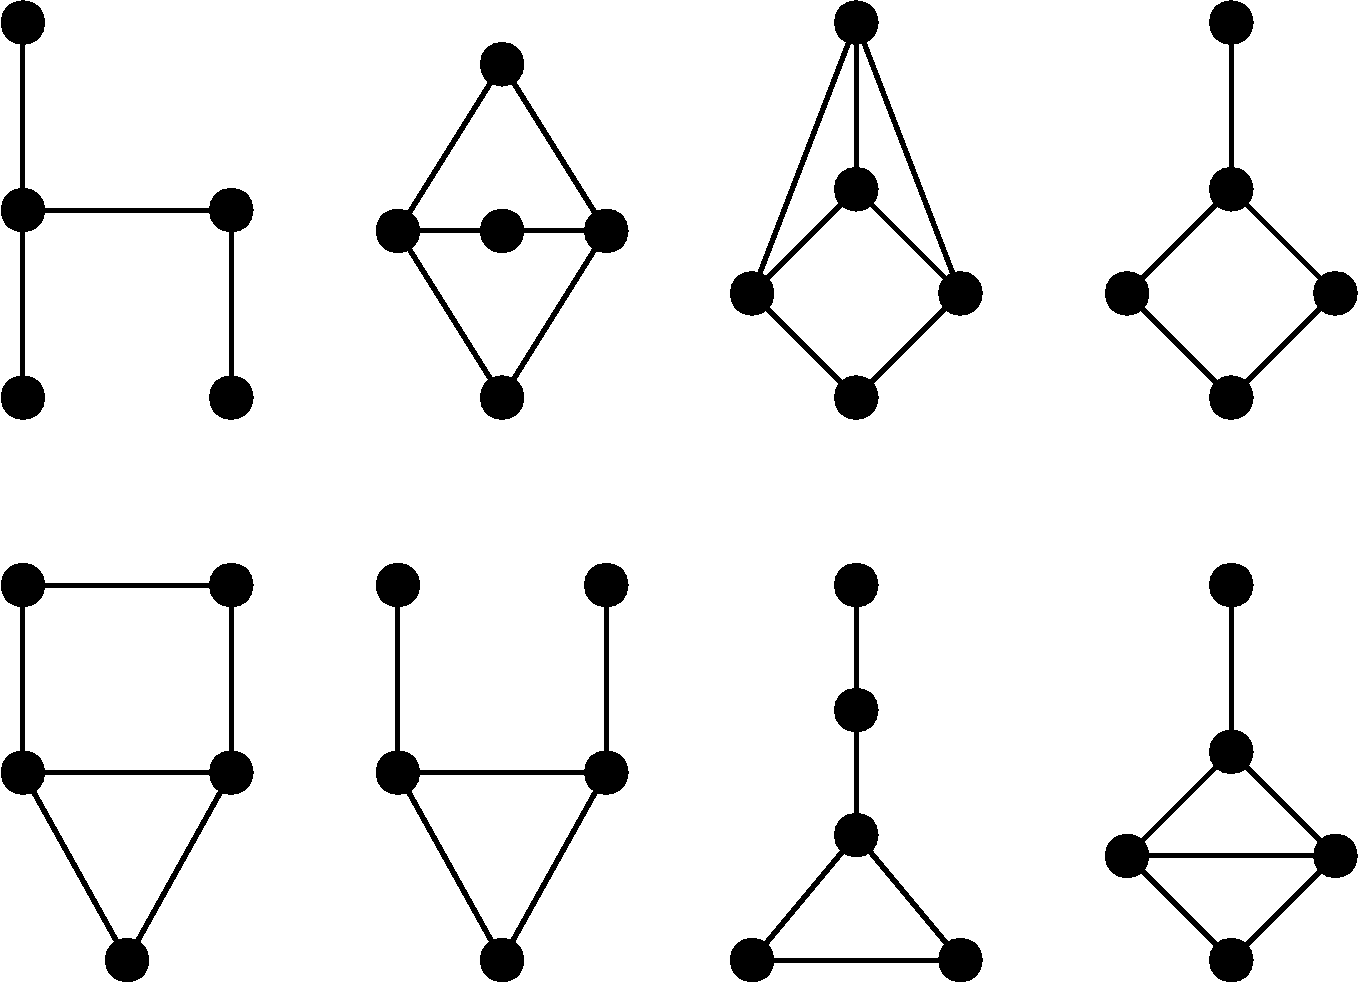
\includegraphics[width=1\columnwidth]{figures/Size5Graphs.pdf}
  \caption{All possible order-3 graphs of 5 nodes.  The room layout shown in Figure~\ref{fig:foldingDiagram} and used in the pilot study corresponds to the top-right graph above.}~\label{fig:size5Graphs}
\end{figure}

Once we allow order 3 (up to three portals per room), the design possibilities expand considerably.  The smallest order-3 graph has four nodes, and there are exactly three such graphs, shown in Figure~\ref{fig:size4Graphs}.  Any arrangement of four rooms, with no more than three portals per room, will be isomorphic to one of these.  Similarly, with five rooms, the layout will be isomorphic to one of the eight graphs shown in Figure~\ref{fig:size5Graphs}.  Larger or higher-order graphs are of course possible too.  While there is in principle no limit to the size or order of the graph layout one could use, order 3 is the smallest order which allows a wide variety of possible designs, and will be taken as a minimal requirement when considering implementation details.

\subsection{Implementation Details}

To implement the space folding technique in VR requires a portal solution that meets the following requirements:

\begin{enumerate}
\item It must work in VR on the platform of choice, allowing users to see through the portal with proper stereo.

\item It must allow for at least three portals in the same virtual space.  Note that it is not strictly necessary to allow for a portal to be visible through another portal; proper arrangement of occluders (e.g. walls) can avoid the need for that.  However, a portal solution that allows for such secondary visibility would reduce constraints on the design of the space.
\end{enumerate}

For this pilot study, the Unity game engine and Oculus Quest headset were chosen.  However, after seeking and evaluating all available off-the-shelf portal solutions, none were found that could meet these criteria.  Most portal solutions did not work in VR at all, or did not work on the Quest; and one allowed for only a single portal.  A custom portal solution was therefore written for this study.

The portals combine a custom shader (see listing in Figure~\ref{lst:worldLimitShader}) with a script to configure materials using that shader for each portal in view.  The shader limits its drawing to a certain region of the world, specified by material properties.  These include $CutPoint$ (a 3D vector), and $CutSign$ (a 4D vector).  For each axis (X, Y, and Z), the shader will use the corresponding element of $CutSign$ to control how drawing is limited relative to $CutPoint$:

\begin{itemize}
\item 1: draw only geometry \textbf{ahead} of $CutPoint$ on this axis
\item 0: don’t cut on this axis (i.e. draw everything)
\item -1: draw only geometry \textbf{behind} $CutPoint$ on this axis
\end{itemize}

In addition, the shade has properties \textit{LineBound1} and \textit{LineBound2}, each a 4D vector, which define two lines in the world.  The fourth element of $CutSign$ controls drawing relative to these lines:

\begin{itemize}
\item 1: draw only to the right of \textit{LineBound1} and left of \textit{LineBound2}
\item 0: don’t limit drawing by the line bounds
\item -1: draw only to the left of \textit{LineBound1} and right of \textit{LineBound2}
\end{itemize}

Each virtual room is assigned a unique material that uses the custom shader.  A script on each portal then configures the materials for its “local” and “remote” rooms as follows: $CutPoint$ is set to the center of the portal; the line bounds are set to the left and right edges of the portal; and $CutSign$ is set so that the remote material is drawn only for the frustum of space through the portal, and the local material is drawn everywhere except that same frustum.

The effect of this shader can be seen in Figure~\ref{fig:shaderEffect}.

\begin{figure}[htb]
  \centering
  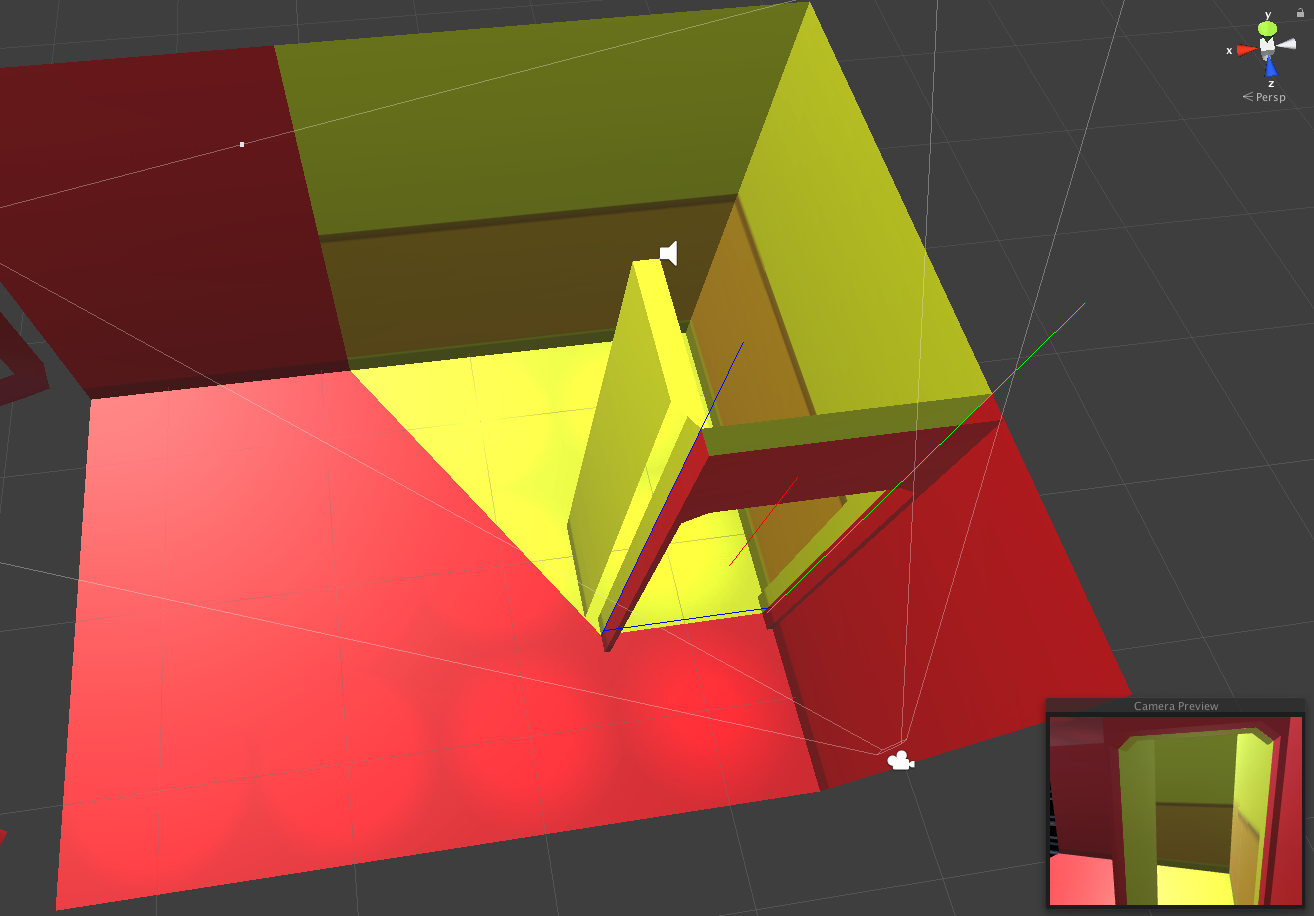
\includegraphics[width=1\columnwidth]{figures/ShaderEffect.png}
  \caption{Effect of the world-limit shader.  Player’s viewpoint is indicated by the camera icon in the corner of the space.  The local material is here tinted red, and the remote (seen through the portal) material is tinted yellow.  Inset shows the view from the player’s perspective.  Tint colors are for illustrative purposes only; in the actual study, all materials were untinted.}~\label{fig:shaderEffect}
\end{figure}


\subsection{Pilot Study}

A small pilot study was done to test the effectiveness of the technique and get initial reactions from users.  The study used the $3 m \times 4 m$ layout shown in Figure~\ref{fig:foldingDiagram}, and was conducted on a workout mat approximately $4 m \times 5 m$, with the Oculus Quest “Guardian” (play area) boundary configured to extend beyond the edges of the mat, so that the boundary feedback grid would not appear as long as subjects stayed within the walls of the virtual space.  Figure~\ref{fig:labSpace} (top) shows the system in use.  Note that Oculus Quest is an entirely wireless system, eliminating the need for wire management that commonly arises in older VR setups.

\begin{figure}[htb]
  \centering
  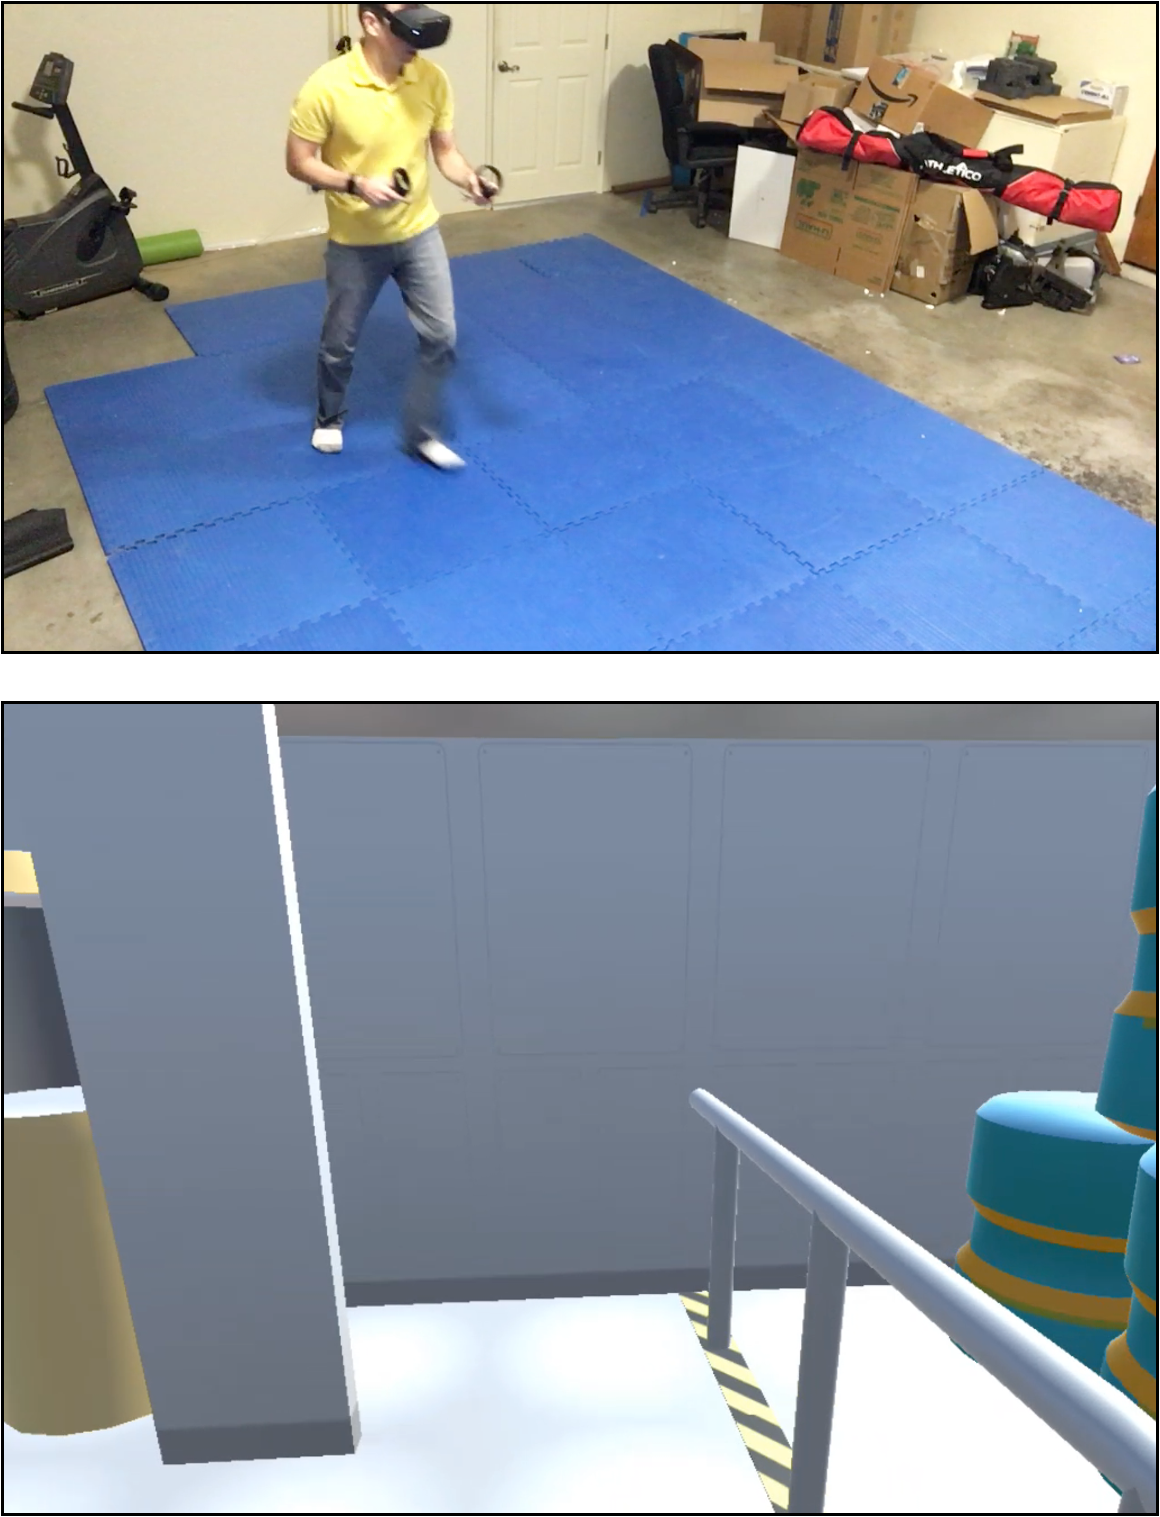
\includegraphics[width=1\columnwidth]{figures/LabSpace.pdf}
  \caption{Image of a user using the system (top), and the corresponding view inside the headset (bottom).}~\label{fig:labSpace}
\end{figure}

The virtual space was modeled and textured to suggest a science-fiction spaceship, with a “cockpit” including a large window at one end, and an “aft” room with a smaller window at the other.  In between were two rooms called “red cargo” and “blue cargo”, decorated with red crates and blue barrels respectively; and the “midship” room, which featured a different wall style and connections to the cockpit and both cargo rooms.  In each room was a round cabinet, labeled near the top with the name of the room.  In one room at a time, a pickup target — a bouncing yellow star — would appear in the cabinet.  The corresponding room label also appeared above the user’s left hand (which appeared in the simulation as the standard Quest controller model).  This is used to inform the user which room contains the pickup star.  In Figure~\ref{fig:labSpace} (bottom), part of the blue cargo room can be seen.

The experimental protocol was as follows.  First, the subject was brought into the experimental space and given a brief introduction to the headset and controllers.  The experimenter then donned the headset to launch the app and adjust the starting position, ensuring that the virtual space was properly positioned within the physical space.  The experimenter then helped the subject put on and adjust the headset, and finally handed the subject both controllers.  The subject was then instructed to observe the label floating over the left controller, find the corresponding cabinet, and touch the floating star with either controller.  On that event, the star disappears with a confirmation sound, reappears in some other room, and the controller label updates accordingly.  Users were instructed to follow these prompts until they had found a star in every room.

Once that was accomplished, the users were given a 5-minute period in which to continue that same task (collecting stars by following the prompts).  They were instructed to collect stars “as quickly as you reasonably can without running.”  No further communication with the experimenter was allowed during the five-minute period, apart from a notification when there was 1 minute remaining.  The experimenter recorded the start and stop time of the trial on the subject data sheet.

After the 5-minute period was up, the subject was stopped, helped out of the VR gear, and given a survey consisting of 7 Likert-scale questions.  This was followed by the (unweighted) NASA TLX (Task Load Index) survey.  Finally, the subject was given an opportunity to provide any free-form comments about the experience.

The study app was written to collect data continuously while running: every 0.1 seconds, it writes a line to a CSV file that includes the time, the headset position and orientation, and any event such as a pickup prompt appearing or a star being collected.  Each data file is timestamped so that it could be matched to subject data sheets.

Five subjects participated in this pilot study.  Three of these were the experimenter’s family; two were friends and neighbors.

\begin{figure*}[htb]
  \centering
  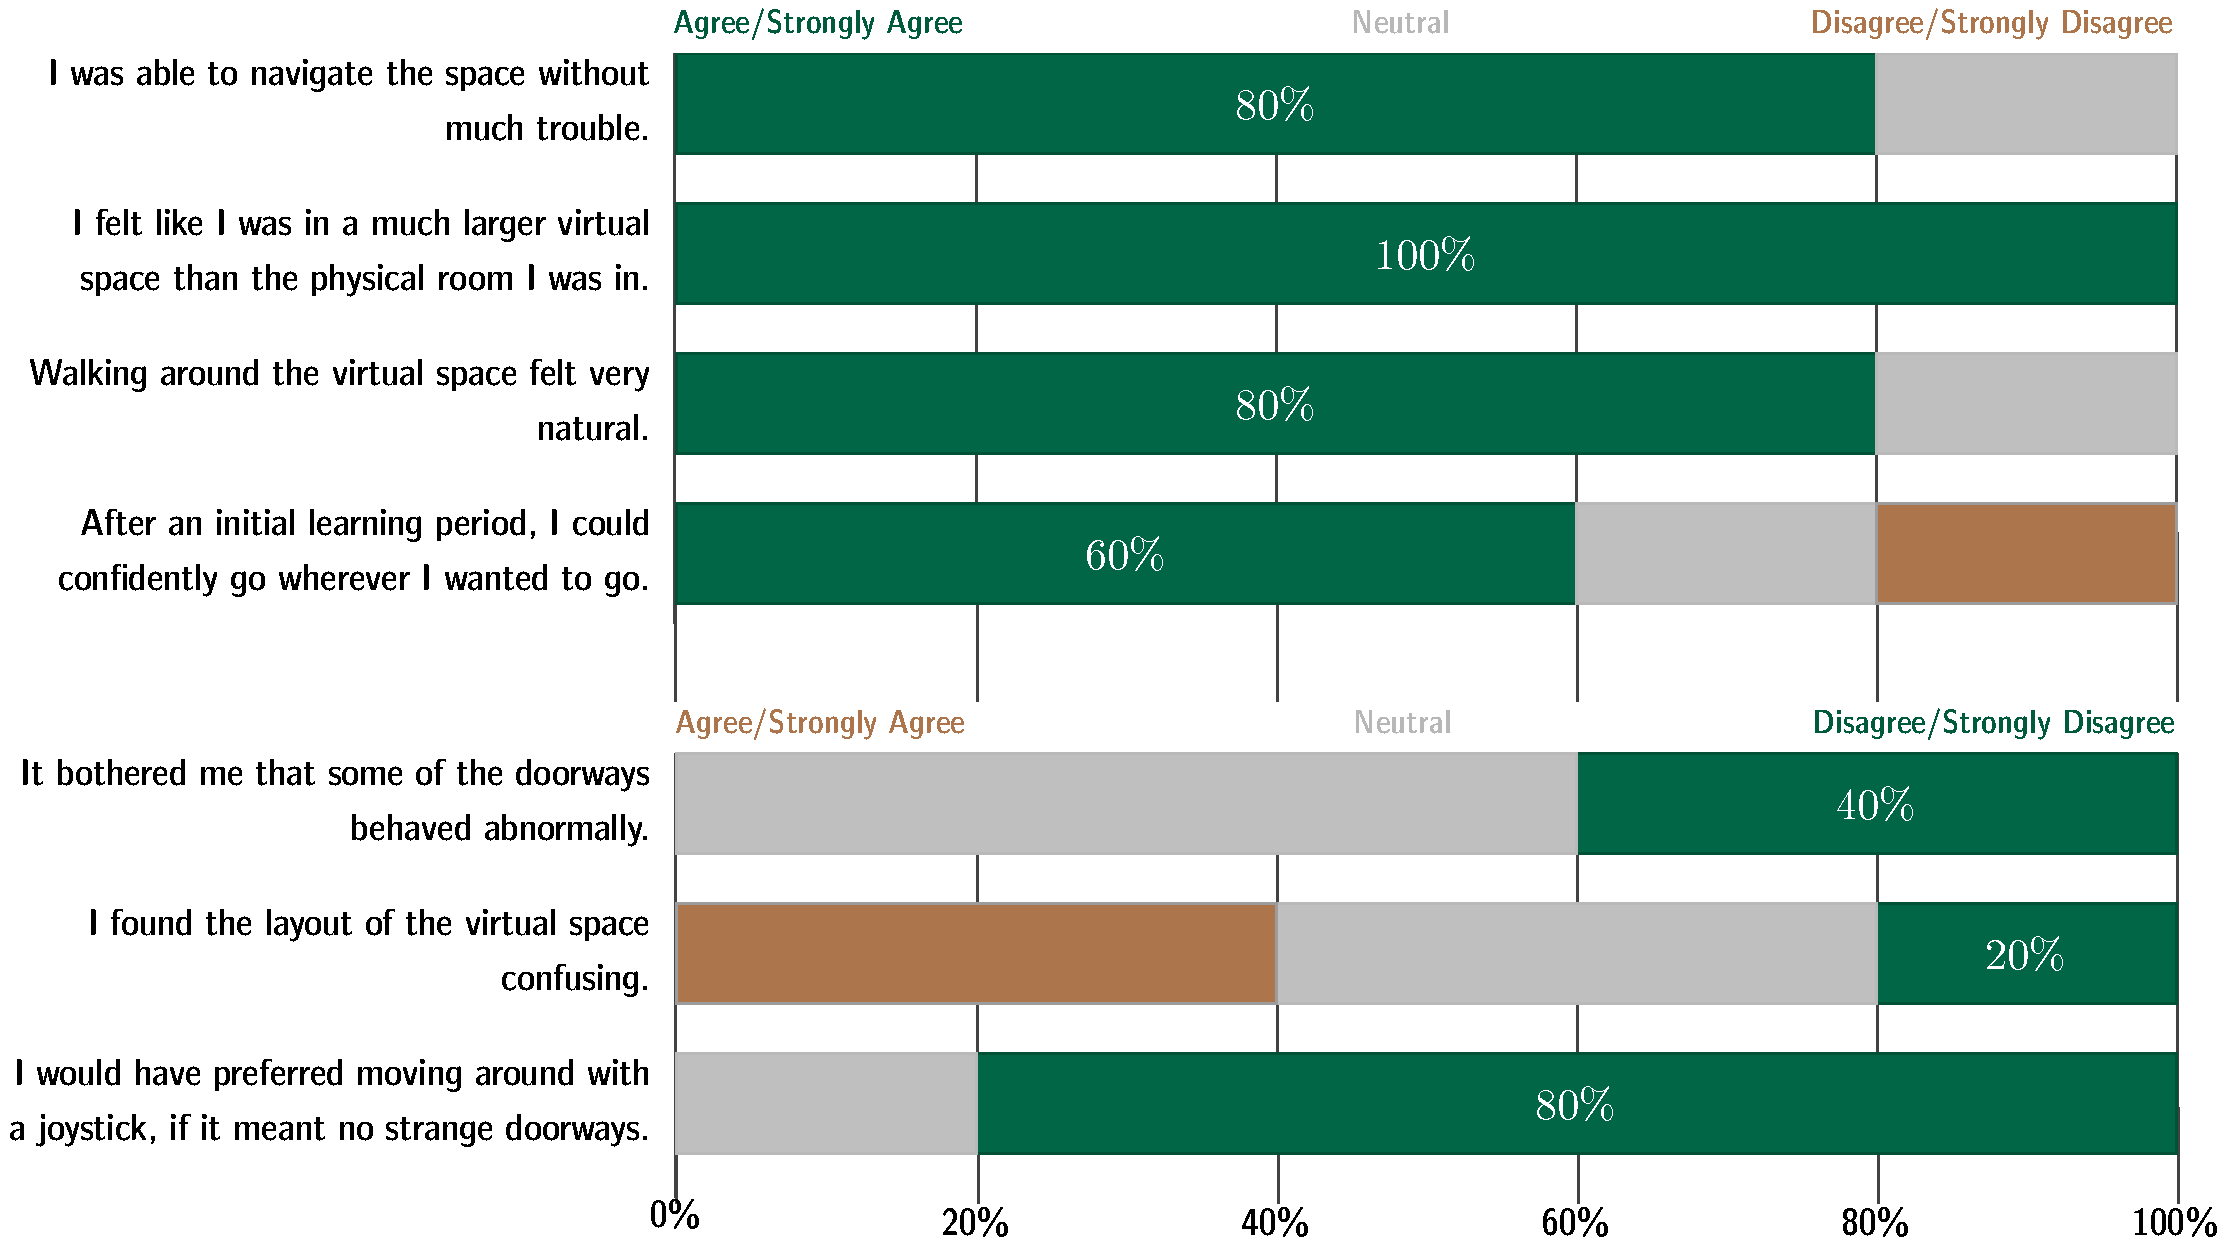
\includegraphics[width=1.75\columnwidth]{figures/LikertChart.pdf}
  \caption{Post-trial survey responses collected in the pilot study.  Positive (top) and negative (bottom) statements have been grouped here, but were interleaved in the actual questionnaire.}~\label{fig:likertChart}
\end{figure*}

\section{Results}

The exit survey questions, and summary of responses, is shown in Figure~\ref{fig:likertChart}.  Note that on the actual survey, positive and negative statements were interleaved, but they have been grouped in the figure for clarity.  Also, though a 5-point Likert scale was used in the survey, we are here grouping “Agree” and “Strongly Agree” for the sake of analysis, and similarly grouping “Disagree” and “Strongly Disagree.”

There was strong overall agreement with the positive statements.  All users agreed with “I felt like I was in a much larger virtual space than the physical room I was in,” and 4 out of 5 users also agreed that “I was able to navigate the space without much trouble” and “Walking around in the virtual space felt very natural,” with the other user in each case remaining neutral.  On “After an initial learning period, I could confidently go wherever I wanted to go,” 3 of 5 users agreed, with one neutral and one disagreeing.

On the negative statements, 4 out of 5 subjects disagreed with “I would have preferred moving around with a joystick, if it meant no strange doorways,” with 1 subject neutral.  On “It bothered me that some of the doorways behaved abnormally,” 2 subjects disagreed, with the other three marking neutral.  However, on “I found the layout of the virtual space confusing,” 2 subjects agreed, 1 disagreed, and 2 were neutral.

\begin{table}[]
\begin{tabular}{lllllll}
\toprule
Scale & S1 & S2 & S3 & S4 & S5 & Median \\ \midrule
Mental Demand & 12 & 14 & 8 & 11 & 13 & 11.5 \\
Physical Demand & 4 & 4 & 2 & 3 & 3 & 3.5 \\
Temporal Demand & 4 & 11 & 3 & 9 & 8 & 6.5 \\
Performance & 7 & 14 & 4 & 8 & 16 & 7.5 \\
Effort & 6 & 15 & 9 & 11 & 13 & 10 \\
Frustration & 6 & 13 & 4 & 3 & 1 & 5 \\ \bottomrule
\end{tabular}
\caption{Raw data from the NASA TLX survey.  Each column S1 - S5 represents the responses of one subject; rightmost column shows median.  All scales are from 1 (low) to 20 (high), except for Performance, which is inverted: 1 represents perfect performance, and 20 indicates failure.}
\label{table:nasaTLX}
\end{table}

The results of the NASA TLX surveys are shown in Table~\ref{table:nasaTLX}.  On each 20-point scale, lower numbers are better, i.e., indicate less task load and more success.

Finally, Table~\ref{table:comments} shows free-form comments collected from the subjects about their experience using the system.

\begin{table}[]
\begin{tabular}{lllllll}
\toprule
“it felt oddly natural” \\
“this shouldn’t feel normal, but it does” \\
“I understood where each of the rooms were” \\
“I could see a discrepancy” \\
“would have liked another 5 minutes or so” \\
“it was a creative use of a limited amount of space” \\
“it had the feel of a Portal game” \\
“I like the simple and easy-to-understand layout” \\
\bottomrule
\end{tabular}
\caption{Free-form comments from the subjects of the pilot study.}
\label{table:comments}
\end{table}

\section{Discussion}

The pilot study suggests that users find the VR space folding technique generally appealing, and, consistent with earlier studies, seem to prefer natural walking as a means of navigating a VE.  Participants unanimously agreed that they had a feeling of being in a larger space, and most agreed that they could navigate the space without trouble.

A key difference between the space folding technique and earlier approaches to spatial compression is that space folding makes no attempt to hide the manipulation from the user.  Users are almost immediately aware that the portals in the VE are not like doorways in real life, and that passing through one leads to another space that overlaps the space they left.  Two respondents indicated in the exit survey that they were bothered by this behavior, but only one respondent found it confusing.  And no subjects indicated they would have preferred joystick travel, if it meant ordinary doorways.

These results support the idea that, while space folding is not hidden from the user, the cost of exposing the spatial manipulation is small, while the benefit (natural walking in a much larger virtual environment) is substantial.

A secondary purpose behind the pilot study was to discover procedural issues that might cause difficulty in a larger experiment.  A few such issues were uncovered.  First, care must be taken to position the VE correctly in the physical environment on the start of each run.  On a few of the trials, this was not done accurately, causing subjects to step off the mat, which is a jarring experience.  Second, one subject wore glasses with progressive lenses (different focal length at the top of each lens compared to the bottom), and found that text high in the visual field was blurry.  On this basis, the labels on each cabinet should be placed on or near the waist-high shelf rather than at the cabinet top, so they can be easily read by all subjects.  Finally, one subject had a fair amount of difficulty adjusting the headset, and several times throughout the trial had to shift the headset, despite having a controller in each hand.  More care should be taken to ensure a good fit for each subject, and since the trial protocol doesn’t really require both controllers, perhaps it should use only one, leaving the other hand free in case it is needed.

On the positive side, the Oculus Quest proved to be a very easy hardware platform to work with, and for at least 4 out of 5 subjects, was very quick to put on and adjust, and apparently comfortable to use.  The lack of any wires is a critical benefit for an experiment like this, where users are walking quickly in often circuitous patterns.  In addition, although there was nothing in the code to prevent users from walking through walls, no subject in the pilot study ever did this (despite no specific instructions to avoid that).  Short-cutting through walls was a potential problem that did not materialze.

In terms of experiment design, the pilot study has some obvious limitations beyond the small sample size obtained.  As there is no control condition, we can’t do any statistical tests of significance, or accept or reject any scientific hypothesis.  Moreover, as the subjects were all friends or family of the experimenter, they cannot be considered impartial; response bias is a very real possibility.  These factors could be improved in a larger, properly controlled study.

On a technical level, the implementation used suffered from a few issues as well.  Something about the custom shader, or perhaps the associated C\# scripts, sometimes caused a noticeable drop in frame rate when a portal was in view.  This resulted in laggy tracking of the head and hand controllers.  While none of the subjects complained about this effect, it was clearly noticeable to the author, and distracts from the smooth VR experience elsewhere in the VE.  Along similar lines, there is often a visual glitch or “flash” as one passes through a portal that the author was unable to track down.  This too distracts from a smooth experience.

Moreover, the approach used in this portal solution has some inherent limitations.  Because it limits the drawing of a material, all objects visible from a portal must use the same material (or another material using the same shader, but that would complicate the update scripts).  This has some performance benefits, in that it limits draw calls, but it placed challenging constraints on the modeling of the VE.  Moreover, the approach breaks down completely if more than one portal is active at a time, which required a rather complex set of triggers and scripts to turn portals (and some other room objects) on and off as the user moved around the environment.  In the final study, all of that was working correctly, but it was onerous to set up and makes the VE difficult to modify.

However, those are limitations of the particular prototype implementation used, not the approach itself.  Considering VR space folding itself, there are several implications and design considerations that may be drawn.

First, a physical space of at least $2 m \times 3 m$ is needed.  This gives room for three portals, assuming each portal needs one square meter on either side to give the user room to walk.  However, at that scale an order-three room will be nothing but doors, and even order-2 rooms feel a bit cramped.  This study used a slightly larger $3 m \times 4 m$ layout, which allows for a comfortable amount of space in each room. That’s somewhat on the large side for home VR setups, but not outrageously so.

Second, space folding works best for indoor scenes, where there are walls to constrain the users and obvious doorways or arches to bound the portals.  It would not be easily applied to a VE that represents an open field, forest, or similar.

Finally, while there is in principle no limit on how much virtual space can be folded into a modest physical space, in practice, frequently walking a long way (by necessity doubling back on your path a number of times) might get tedious.  However, it’s important to note that shortcuts are quite possible; the rooms do not need to be arranged in any neat Euclidean order.  One could have portals from one end of the VE that connect directly to the other end, or virtual elevators that one steps into and presses a button, causing the portal to connect to a different section of the VE entirely.  With the addition of these techniques, an arbitrarily large VE could be traversed efficiently.
	
\section{Conclusion}

This study presents a new approach to spatial compression in virtual reality called VR space folding.  It allows users to walk around an arbitrarily large virtual environment in a physical space as small as $2 m \times 3 m$.  Unlike most previous techniques, it makes no attempt to prevent users from noticing the spatial manipulation, which takes the form of portals that connect one virtual room to another (using the same physical space).  

To assess whether this spatial manipulation confuses or annoys users, a small pilot study was done.  Survey responses from study participants indicate that, on the whole, they did not find the folded space confusing, and appreciated the freedom to traverse it naturally via real walking.  Because this technique allows for large spatial gain in a space small enough to fit in many home VR setups, it has the potential to be a very useful technique for a wide variety of VR applications, though with the caveat that it works best for indoor (rather than outdoor) environments.

Future work should further validate these results by doing a larger, controlled study.  For example, one could compare subject’s effectiveness in collecting targets under three conditions: folded space with natural walking, folded space with joystick travel, and unfolded space with joystick travel.  A comparison of the first two would reveal any significant difference between walking and joystick travel, while the second two conditions would reveal any difference between folded space and unfolded space.  Based on the preliminary results of this pilot study, one might expect a significant advantage to walking over joystick travel, but no significant difference between unfolded space and folded space.  Put together, this would strongly indicate the benefit of combining folded space with natural walking in any case where a larger VE than the physical space is wanted.

\section{Acknowledgments}

The author wishes to thank Francisco Ortega and Aditya Raikwar, both at Colorado State University, for their encouragement and feedback on early versions of the prototype.

\begin{figure*}
\lstinputlisting[language=C]{WorldLimit.shader}
  \caption{Source code for the world-limit shader used as the key component of the custom portal solution used in the pilot study.}~\label{lst:worldLimitShader}
\end{figure*}


% Balancing columns in a ref list is a bit of a pain because you
% either use a hack like flushend or balance, or manually insert
% a column break.  http://www.tex.ac.uk/cgi-bin/texfaq2html?label=balance
% multicols doesn’t work because we’re already in two-column mode,
% and flushend isn’t awesome, so I choose balance.  See this
% for more info: http://cs.brown.edu/system/software/latex/doc/balance.pdf
%
% Note that in a perfect world balance wants to be in the first
% column of the last page.
%
% If balance doesn’t work for you, you can remove that and
% hard-code a column break into the bbl file right before you
% submit:
%
% http://stackoverflow.com/questions/2149854/how-to-manually-equalize-columns-
% in-an-ieee-paper-if-using-bibtex
%
% Or, just remove \balance and give up on balancing the last page.
%
\balance{}

% REFERENCES FORMAT
% References must be the same font size as other body text.
\bibliographystyle{SIGCHI-Reference-Format}
\bibliography{sample}

\end{document}

%%% Local Variables:
%%% mode: latex
%%% TeX-master: t
%%% End:
